\documentclass[10pt]{article}
\usepackage[margin=1.2in]{geometry}

%\usepackage{algpseudocode}
%\usepackage{algorithm}

\usepackage{graphicx}
\usepackage{fmtcount}

\usepackage{multirow}

\usepackage[hyphens]{url}
\usepackage{hyperref}

\usepackage{array}
\usepackage{amsmath}
\usepackage{amssymb}

%\usepackage{natbib}

\usepackage{mathtools}

\usepackage{listings}
\usepackage{color}
\usepackage{booktabs}

% keywords: fixme

\sloppy

\begin{document}

\title{Practically efficient methods for performing bit-reversed
  permutation in {\tt C++11} on the {\tt x86-64} architecture}

\author{Christian Knauth\\
Freie Universit\"at Berlin\\
Institut f\"{u}r Informatik
\and
Boran Adas\\
Freie Universit\"at Berlin\\
Institut f\"{u}r Informatik
\and
Daniel Whitfield\\
Freie Universit\"at Berlin\\
Institut f\"{u}r Informatik
\and
Xuesong Wang\\
Freie Universit\"at Berlin\\
Institut f\"{u}r Informatik
\and
Lydia Ickler\\
Freie Universit\"at Berlin\\
Institut f\"{u}r Informatik
\and
Tim Conrad\\
Freie Universit\"at Berlin\\
Institut f\"{u}r Informatik
\and
Oliver Serang\\
Freie Universit\"at Berlin\\
Institut f\"{u}r Informatik\\
\url{orserang@uw.edu}
}

\date{{\small \today}}

\maketitle

\begin{abstract}
\noindent La permutación invertida con “bits” es una problem famosa en la señal procesamiento y es clave para la implementación eficiente de FFT. Este artículo presenta implementaciones optimizadas {\tt C++11} De cinco métodos existentes para calcular la permutación invertida en bits: “Stockham auto-sort”, intercambio de bits ingenuo, intercambiando a través de una tabla de Bytes invertidos, intercambio local de bits por pares, e intercambio a través de un Tampón de matriz localizado en caché. Tres nuevas estrategias para la Se invierte la permutación de bits invertida en {\tt C++11}: una inductiva utilizando la operación XOR bit a bit, una plantilla recursiva cerrada forma, y ​​un acercamiento esquemático-recursivo de memoria caché, que reduce la permutación invertida en bits a las permutaciones de bits invertidos menores y una transposición matricial cuadrada. Estos nuevos métodos se comparan con los enfoques existentes en términos de tiempo de ejecución teórico, compilación empírica tiempo y tiempo de ejecución empírico. La plantilla-caché recursivo-olvidadizo se muestra que es competitivo con el método más rápido conocido. Sin embargo, se demuestra que el método caché-olvido puede más se benefician fácilmente de la paralelización en múltiples núcleos y en la GPU.
\end{abstract}

\section*{Introdución}
La clásica transformada de Fourier rápida de Cooley-Tukey (FFT) funciona
Reducir de forma recursiva una FFT a dos FFT de la mitad del tamaño (en el caso de diezmación en el tiempo estos FFTs más pequeños se evalúan en el par
Los índices y los índices impares del original array)\cite{cooley: algoritmo}. Cooley-Tukey es muy importante para
Sus múltiples aplicaciones en la informática científica: por ejemplo, la FFT
Cálculo numérico de la convolución de dos matrices de longitud $ n $ en
$O(n \ log (n))$ pasos en lugar de los $O(n ^ 2)$ requeridos por el ingenuo algoritmo de convolución\cite{proakis: introducción}. La sencillez, eficiencia y la amplia utilidad del trabajo de Cooley y Tukey ser uno de los métodos de informática más influyentes de la \ordinalnum{20} century\cite{cipra:best}.

La forma más sencilla de calcular la FFT Cooley-Tukey es calcularla
Fuera de lugar y utilizando un búfer de tamaño $ n $. Luego, los valores de la matriz original se puede copiar en diferentes índices de la memoria que los índices pares de la matriz se copian a índices $0, 1, \ldots \frac {n} {2}-1$ del búfer y para que los índices impares de la matriz
Se copian a los índices $\frac{n}{2}, \frac{n}{2}+1, \ldots n-1$ de la
buffer. Este enfoque tamponado se conoce comúnmente como "Stockham
Auto-sort” \cite {cochran: fast}.
El cálculo de una FFT en el lugar (\emph{i.e.} Computación de una FFT por
Sobrescribir la matriz evaluada, sin necesidad de un buffer de resultados) es
más desafiante. La permutación par-impar realizada por el Stockham
FFT es equivalente a una matriz $\frac{n}{2} \times 2$
transposición. Por ejemplo, si $n = 8$, entonces los índices $[0, 1, 2, 3, 4, 5, 6, 7]$ puede ser pensado como una matriz $4 \ times 2$, cuyo la transposición corresponde a la deseada permutación par-impar:
\[ 
\left[
  \begin{matrix}
    0 & 1\\
    2 & 3\\
    4 & 5\\
    6 & 7
  \end{matrix}
\right]^T = 
\left[
  \begin{matrix}
    0 & 2 & 4 & 6\\
    1 & 3 & 5 & 7
  \end{matrix}
\right],
\]
Donde los valores de índice par están ahora en la primera fila y el índice impar
Los valores están ahora en la segunda fila. Esta transposición es la inversa de
El shuffle faro (también conocido como “shuffle perfecto”)\cite{sedgewick: algorithms}, en el que se corta una baraja de cartas en la mitad y entonces las dos mitades se entrelazan. FFT en el lugar requiere estas transposiciones de matriz que se realizará en su lugar (\emph{i.e.},
Transponiendo las matrices mientras usan sustancialmente menos de $n$
Memoria adicional); No obstante, la transposición in situ de
Matrices es un desafío porque el índice de destino se escribe
No cambia necesariamente con el valor fuente (como sería el caso
Con una matriz cuadrada). Para transponer una matriz $M \times N$ usando más $O(M + N)$ espacio, los algoritmos existentes requieren runtime $\in
\Omega (M N \log(M N))$\cite{fich: permuting}. Además, incluso si
Rápido $O(n)$ algoritmo estaban disponibles para realizar el par impar
Permutación sin asignación significativa de memoria (quizás explotando el hecho de que se trata de un caso especial de matriz transposición, donde el número de filas y columnas son ambos poderes de dos), realizando esta permutación se separa la FFT de longitud $n$ desde las FFTs recursivas de longitud $\frac{n}{2}$. Esto puede tener una influencia negativa y evitar que el compilador reconozca código en las llamadas recursivas, como las llamadas trigonométricas reutilizadas.Constantes Código FFT que puede ser optimizado por el compilador es altamente valorado y puede producir una aceleración considerable \cite{myrnyy: simple}.
Un enfoque consiste en realizar las permutaciones impares de todos los
Llamadas recursivas al inicio de la FFT. Cada permutación par-impar puede
Ser considerado como la parte menos significativa en la mayoría
Bit significativo, y por lo tanto realizar todos ellos secuencialmente es
Equivalente a permutar intercambiando los índices con su bit a bit
Índices invertidos. La "permutación invertida en bits" de $[0, 1, 2, 3, 4, 5, 6, 7]$ (o $[000, 001, 010, 011, 100, 101, 110, 111]$ en binario)
Sería $[0, 4, 2, 6, 1, 5, 3, 7]$ (o $[000, 100, 010, 110, 001, 101, 011, 111] $ en binario). Dada una función {\tt rev} que invierte indices enteros bit con bit, la permutación invertida en bits es bastante sencillo de realizar ({\bf Listing~\ref{alg: simple-permutación}}). Tenga en cuenta que el bit invertido permutación se puede realizar en el lugar simplemente intercambiando el índice y pares de índices invertidos. Esto es menos complicado que en el lugar transposición de una matriz no cuadrada, ya que se garantiza que {\tt rev(rev(i)) = i}(de una manera similar a la matriz cuadrada transposición). Después de aplicar una permutación invertida, la FFT puede simplemente invocando una versión ligeramente reescrita de la
FFT, que ahora pueden asumir que en cada nivel de recursión, el
Incluso-impar permutación ya se ha realizado.
\begin{footnotesize}
  \lstset{language=C++,
    basicstyle=\ttfamily,
    keywordstyle=\color{blue}\ttfamily,
    stringstyle=\color{red}\ttfamily,
    commentstyle=\color{magenta}\ttfamily,
    morecomment=[l][\color{magenta}]{\#},
    breaklines=true,
  }
\begin{lstlisting}[label={alg:simple-permutation},caption={{\bf Performing the bit-reversed permutation with the help of an external {\tt rev} function.} Let {\tt LOG\_N} be the problem size, which is a {\tt constexpr} (\emph{i.e.}, it is known a constant known at compile time). Note that the function {\tt rev} is templated to take the word size used for reversal.}]
void naive_bitwise_permutation(T*__ restrict const v) {
  constexpr unsigned long int N = 1ul << LOG_N;

  for (unsigned long index=1; index<(N-1); ++index) {
    unsigned long reversed = rev<LOG_N>(index);

    // Comparison ensures swap is performed only once per unique pair (otherwise, every index will be swapped and then swapped back to re-create the original array):
    if (index<reversed)
      std::swap(v[index], v[reversed]);
  }
}
\end{lstlisting}
\end{footnotesize}

Aunque algunos procesadores de señales digitales (DSPs) proporcionan bit nativo operaciones de reversión, muchas CPUs de escritorio modernas (incluyendo la {\tt x64} CPUs al momento de la publicación), no tienen un código de operación para
{\tt rev} función; Por lo tanto, funciones eficientes para calcular {\tt rev} son necesarios. Por supuesto, la inversión de bits puede realizarse a bit en $\Theta(b)$, donde $n=2^b$ que $b$ corresponde a {\tt LOG\_N} en el código de {\tt C++}. Realización de la totalidad del bit invertido
Permutación utilizando este método de inversión de bits ingenuo,
$\Theta(n b) = \Theta(n \log(n))$ pasos.
\paragraph{Bytewise bit reversal:}
Debido a que la función de inversión de bits {\tt rev} se llama en cada índice, optimizar la función {\tt rev} puede ser muy beneficioso para
actuación. Una forma de realizar una inversión de bits significativamente más rápida que el enfoque ingenuo bit a bit es intercambiar con bloques de bytes en lugar de bits Esto se logra eficazmente mediante la codificación de una matriz de {\tt unsigned char}, que contiene 256 entradas, una para cada uno posible byte. Para cualquier byte {\tt B}, el acceso a la tabla en índice
{\tt B} devuelve el valor invertido en bits de ese byte \cite{j: best, anderson: bit}. Con esta tabla de bytes invertida, el mismo enfoque que
Se puede usar el método de bits naive, que requiere $\frac{b}{8}$ pasos en lugar de los $ b $ pasos requeridos por el método bit a bit naive. Esta
Bytewise método es mucho más rápido en la práctica, a pesar de que su asintótico runtime, como el método bitwise ingenuo, sigue siendo $\in \Theta(n \log(n))$.
Incluso si la función de inversión de bits {\tt rev} era nativa
Soportado y funcionado en $ O (1) $ ciclos del reloj de la CPU, el no secuencial los accesos de memoria realizados por la permutación de inversión de bits no se almacenan en caché utilizando el modelo de caché jerárquico estándar (que carga contiguos en el caché cada vez que un valor no almacenado en caché es de la siguiente capa de la jerarquía de la memoria), que es {\tt x64} equipos. Esto contrasta con el otro código FFT, que acceso a la memoria de una manera casi perfectamente secuencial (y caches muy efectivamente). Como resultado, el coste de calcular una grandes FFT puede pasar un porcentaje significativo de su tiempo realizando la permutación invertida en bits.
\paragraph{Reversing bitwise using pairs of bits:}
Un método para lograr un rendimiento de cache mejor se desarrolla a
Trabajando 2 bits a la vez (intercambiando los más significativos y los menos
Bits significativos). Entonces, en lugar de calcular la totalidad del bit invertido indice y luego cambiando si {\tt index < rev(index)}, este par
Bitwise realiza varios swaps, uno después de cada par de bits
Se intercambian \cite{perez: place}. Así, un mayor número de permutas
La matriz se realizan, pero los swaps logran una mejor
localidad. Aunque los bloques de acceso a la memoria no son
Secuencial, son más contiguas que en el ingenuo bit a bit y
Bytewise se acerca. A pesar del mayor número de operaciones de swap
En la matriz, el tiempo de ejecución asintótico de este enfoque no es
Diferente del enfoque de inversión de bits ingenuo, y es, por tanto $\in
\Theta (n \log(n))$.
\paragraph{Bit reversal using a matrix buffer:}
Carter \ & Gatlin propuso un método de optimización de caché que utiliza una matriz buffer. La idea principal es que el tampón es lo suficientemente pequeño para caber completamente dentro de la caché {\ tt L1} o {\ tt L2}, y así el buffer puede accederse en orden de fila mayor o mayor de columna y todavía lograr un buen rendimiento de caché. Dado {\ tt índice = x y z} donde el las cadenas de bits {\tt x} y {\tt z} tienen el mismo tamaño $\log(\sqrt{t})$, su método utiliza un buffer de matriz de tamaño $\sqrt{t} \times \sqrt{t} = T$ \cite{carter: towards}.
Because {\tt rev(index) = rev(z) rev(y) rev(x)}, an out-of-place
method for performing the bit-reversed permutation would copy
$\forall$~{\tt x},~$\forall$~{\tt y},~$\forall$~{\tt z},~{\tt
  dest[rev(z)~rev(y)~rev(x)]~$\gets$~source[x~y~z]}. The method
(denoted COBRA in\cite{carter:towards}) proceeds in two steps: 

\noindent $\forall$~{\tt y},\\
\mbox{} \quad $\forall$~{\tt x},~$\forall$~{\tt z},~{\tt
  buff[rev(x)~rev(z)]~$\gets$~source[x~y~z]}\\
\mbox{} \quad $\forall$~{\tt x},~$\forall$~{\tt z},~{\tt
  dest[z~rev(y)~x]~$\gets$~buff[x~z]}.\\

\noindent This can be modified slightly:

\noindent $\forall$~{\tt y},\\
\mbox{} \quad $\forall$~{\tt x},~$\forall$~{\tt z},~{\tt
  buff[rev(x)~z]~$\gets$~source[x~y~z]}\\
\mbox{} \quad $\forall$~{\tt x},~$\forall$~{\tt z},~{\tt
  dest[rev(z)~rev(y)~x]~$\gets$~buff[x~z]}.\\

Although Carter \& Gatlin describe an out-of-place implementation
(meaning that it writes to {\tt dest} rather than modifying {\tt
  source}), it is possible to adapt the method to an in-place version
by swapping data with {\tt buff} rather than simply copying to or from
{\tt buff}. This requires a third looping step to propagate the
changes made to the buffer back into the array. Note that even this
``in-place'' variant of COBRA still requires a buffer, and so it is
not truly an in-place method.

Assuming a $\Theta(b)$ {\tt rev} method, the asymptotic runtime of
COBRA can be found as follows: The $\forall$~{\tt y} loop requires
$\frac{n}{t}$ steps, and the $\forall$~{\tt x} and $\forall$~{\tt z}
loops each require $\sqrt{t}$ steps. By caching bit-reversed values
(\emph{e.g.}, {\tt rev(y)}) as soon as they can be computed, the
runtime is
\[
\underbrace{\frac{n}{t} \cdot }_{\forall~{\tt y}} \left( \underbrace{ \log(\frac{n}{t}) }_{\mbox{\footnotesize Computing {\tt rev(y)}}} +~ \underbrace{2 \cdot}_{\mbox{\footnotesize Copy to/from {\tt buff}}} \underbrace{\sqrt{t}}_{\forall~{\tt x}} \left(
\underbrace{\log(\sqrt{t})}_{\mbox{\footnotesize Computing {\tt rev(x)} or {\tt rev(z)}}} + \underbrace{\sqrt{t}}_{\forall~{\tt z}} \right) \right).
\] asymptotically, this runtime is $\in \Theta\left( n + \frac{n}{t}
\log(\frac{n}{t}) \right)$. Note that using a large buffer
(\emph{i.e.}, $t \gg 1$), the runtime approaches $\Theta\left( n
\right)$ however, this is achieved by sacrificing the improved cache
performance that can be achieved when $t$ is small enough to fit into
the {\tt L1} or {\tt L2} cache. Conversely, when $n \gg t$, then the
runtime will be $\in \Theta(n \log(n))$. Unlike cache-oblivious
methods, which perform well for any hierarchical caches, for any
problem size $n$, the COBRA algorithm needs to optimize the parameter
$t$ for a particular architecture.

COBRA has previously been demonstrated to outperform a method from
Karp\cite{carter:towards}; before that, Karp's method had been shown
to outperform 30 other methods\cite{karp:bit}.\newline

En este trabajo introducimos tres métodos adicionales para realizar la
Permutación invertida en bits. A continuación, se comparan las
Rendimiento práctico a los métodos existentes mediante el benchmarking rápido
Implementaciones de todos los métodos en {\tt C++11}.

\section*{Methods}

\paragraph{Inductive XOR method for generating bit-reversed indices:}
En primer lugar proponemos un método que evita llamar a la función {\tt rev}
en total. Esto se logra mediante la generación inductiva
Índices de bits invertidos sin el uso de invertir en bits o bytewise
Invirtiendo con una tabla de bytes invertida.

Comience con el primer índice y su valor invertido: {\tt index = rev(índice) = 0}. El siguiente índice puede ser trivialmente calculado como {\tt index + 1}, pero el siguiente índice invertido se encuentra vía {\ tt rev(index + 1)}, que no necesariamente será igual a {\ tt rev(index)+1}. En lugar de llamar explícitamente a una función {\tt rev}
(Ya sea bit a bit o bytewise), evitamos esto haciendo uso de
La función XOR bit a bit. {\tt index} XOR {\tt index + 1} sólo revela
Los bits que han cambiado por incrementar. Invertir ambos {\ tt índice}
Y {\tt índice + 1} y computación {\tt rev(índice)} XOR {\tt rev(index + 1)} será equivalente a computación {\tt rev(} {\tt index}
XOR {\tt índice + 1)}, porque la operación XOR bit a bit no
Intercambiar cualquier información entre bits. Además, {\tt index} XOR
{\tt index + 1} reflejará el hecho de que todos los bits diferentes reflejan una
Operación de transporte en adición binaria; Por lo tanto, {\tt index} XOR {\tt index + 1} debe ser de la forma {\tt 000 \ldots 0111 \ldots 1}. Un poco
La cadena de esta forma se puede invertir eficientemente simplemente cambiando por el número de ceros a la izquierda, produciendo así una cadena de bits del formulario {\tt 1 \ldots 1110 \ldots 000}. el número de ceros a la izquierda en una cadena de bits de $ b $ bits puede ser
Calculado trivialmente en $O(b)$ pasos, pero también se puede calcular en
$O(\log(b))$ pasos. Un $O(\log(b))$ runtime se logra por
Bitmasking con una cadena de bits con el más significativo $\frac{b}{2}$
Igual a 1 y el menos significativo $\frac{b}{2}$ bits igual a 0,
Descubriendo con ello la mitad que contiene un bit de 1. La primera mitad con un 1 se puede subdividir iterativamente para encontrar el más significativo 1 en $O(\log(b))$ steps \cite{anderson: bit}.

El número de ceros iniciales también se puede calcular en $O(1)$ a través del
Integer $\log_2$: esto se puede realizar mediante casting a un flotador y
Bitmasking para recuperar el exponente; Sin embargo, este enfoque sólo funciona para $b \leq 24$ \cite{anderson: bit}. Para problemas grandes con $b>24$, que la deficiencia se puede resolver mediante el casting a {\ tt doble}, aunque “casting” a {\tt doble} sería menos eficiente. Afortunadamente, incluso aunque la arquitectura {\tt x64} no tiene un opcode para realizando {\tt rev} en $O(1)$, tiene un opcode para calculando el número de ceros iniciales. En {\tt g++} y {\tt clang}
Esto se puede acceder a través del nombre {\ tt \_ \_ builtin \_clzl} (que
Cuenta los ceros a la izquierda en un {\tt unsigned long int}).

Como resultado, se puede invertir {\tt rev(index)} XOR {\tt rev(index + 1)}
En muy pocas operaciones calculando los bits que difieren entre {\tt rev(index)} y {\tt rev(index + 1)}. El siguiente índice invertido, {\tt rev (index + 1)}, se calcula volteando sólo aquellos bits
Que difiere de {\tt rev(index)} usando XOR ({\bf figura~\ref{figura: xor}}). El método XOR realiza un número constante
De operaciones XOR, así como un solo conteo que lleva la operación de ceros a
Calcular el índice siguiente y el índice invertido. Cuentan los ceros principales
$\in \Theta(\log(b)) = \Theta(\log(\log(n))$ en el
Caso general, y se puede realizar en $O(1)$ cuando $b \leq 24$ o cuando
Soporte de hardware una operación incorporada. Así, el tiempo de
La permutación de bits invertida completa será $\in \Theta(n \log(\log(n))$ in el caso general y $\in \Theta(n)$ cuando se cuentan los ceros iniciales puede ser realizado en $O(1)$.

\begin{figure}
\centering
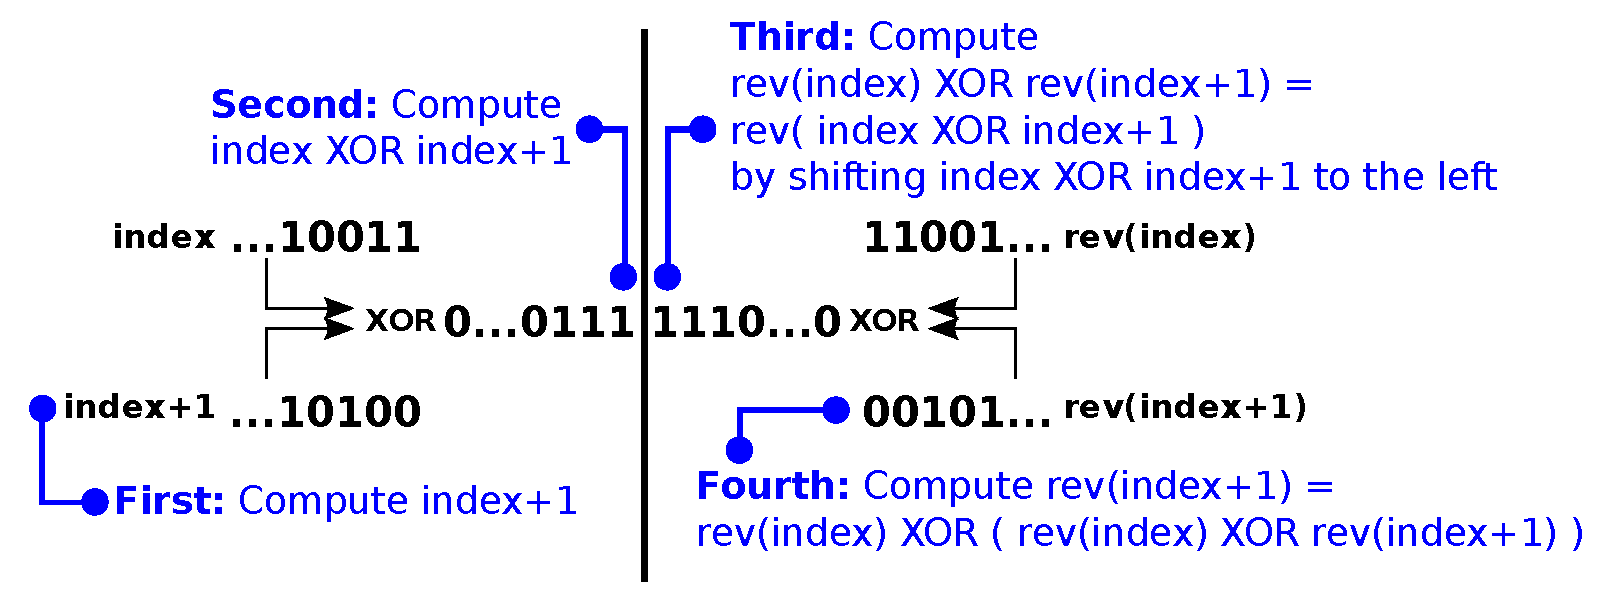
\includegraphics[width=6in]{cartoons/xor.pdf}
\caption{{\bf Illustration of the inductive XOR method for bit
    reversal.} Beginning with {\tt index} and its bit-reverse value
  {\tt rev(index)}, the next values ({\tt index+1} and {\tt
    rev(index+1)}) are computed. First, {\tt index+1} is
  computed. Second, the bits that are different between {\tt index}
  and {\tt index+1} are computed via XOR; the resulting bit string
  will be of the form {\tt 000\ldots 0111\ldots 1}. Third, because the
  differing bits will be of the form {\tt 000\ldots 0111\ldots 1},
  they can be reversed by bit shifting left by the number of leading
  zeros. Fourth, {\tt rev(index+1)} can be computed by flipping only
  the differing bits (via XOR). 
  \label{figure:xor}}
\end{figure}

El método XOR es muy eficiente al calcular el siguiente índice y al siguiente
Índice invertido; Sin embargo, incluso si ese cálculo fuera instantáneo,
El algoritmo sólo alcanza un rendimiento moderado por dos razones:
Primera razón es que no se accede a los índices invertidos en un
De manera contigua (y por lo tanto no se optimizan en caché). El segundo
Razón es la declaración de {\tt if}, que también se encuentra en {\bf Listing~\ref{alg: simple-permutation}}. Esta declaración {\tt if}
Que el desenrollado de bucles sea totalmente efectivo, porque
El compilador no sabrá todavía los efectos de la permutación en el
Iteración (limitando la posibilidad de intercambiar en paralelo, aunque el hardware
Lo apoyaría). También debe tenerse en cuenta que la frecuencia
Que {\tt index < rev(index)} cambiará durante el bucle,
Disminuyendo los beneficios de la predicción de ramas.
\paragraph{Unrolling (template-recursive closed form):}
Eliminar la comparación {\tt if(index < rev(index))} es difícil,
Porque requiere computar anticipadamente los índices sobre los cuales
Será verdad y luego sólo visitará esos índices; Correctamente informando
El patrón de índices donde esto es cierto es sorprendentemente similar a
Realizando inversión de bits. Sin embargo, para problemas de tamaño fijo
(\emph{p. Ej., $B = 10$ bits o equivalentemente $n = 1024$), es
Posible calcular simplemente todos los índices que deben ser intercambiados
Permutación invertida en bits. Esto ofrece dos ventajas: Primero, el
Sobrecarga de bucle, realizar la inversión de bits en los índices, y
Verificando si {\tt index <rev(index)} son todos eliminados. Segundo,
El compilador podría (en teoría) reorganizar las operaciones de swap para ser
Más secuencialmente contiguas, mejorando así el rendimiento de la memoria caché.

Esto podría implementarse a través de una función de código fijo {\tt desenrollado \_permutation \_10}, pero alternativamente también podría ser
Implementado generando ese código en tiempo de compilación a través de la plantilla
Recursión Para cualquier cadena de bits de la forma {\tt index = z x y} (donde
{\tt z x y} es la concatenación de las cadenas de bits {\tt z}, {\tt x}, y
{\tt y}), el inverso será {\ tt rev(index) = rev(y) rev(x) rev (z)}. Cuando las cadenas de bits {\tt z} y {\tt y} consisten en solo bit, entonces su inversión puede ser ignorada: {\tt rev(index) = y rev (x) z}. Así, es posible partir de ambos extremos (el bit más significativo restante y el bit menos significativo restante) y proceder hacia adentro para generar recursivamente problemas de la misma forma (Estas llamadas recursivas se implementan a través de la recursión de plantilla a desenrollarlos en tiempo de compilación). Algunas de las recurrencias de plantilla pueden ser
Abortado en un estilo de rama-y-atado ({\bf
  Figura~\ref {figure: unrolled}}): Cadenas de bits de la forma {\tt index =
  1 ~ x ~ 0} nunca será menor que su reverso, independientemente del
Valor de la cadena de bits {\tt x}; Por lo tanto, una recursión adicional puede ser abortado. Del mismo modo, las cadenas de bits de la forma {\tt index = 0 ~ x ~ 1} siempre será menor que su reverso, y por lo tanto las operaciones de swap debe realizarse para cada posible {\ tt x}. Por último, las secuencias de bits de la forma {\ tt 0 ~ x ~ 0} y {\ tt 1 ~ x ~ 1} será menor que su reverso cuando {\ tt x <rev (x)}. Esto produce un problema de la misma forma que encontrando si {\ tt index <rev (index)}, pero dos bits más pequeños, y por lo tanto se puede realizar recursivamente.
As a result, the runtime of this method is defined by the recurrence
$r(b) = \underbrace{2^{b-2}}_{green} + \underbrace{2 \cdot
  r(b-2)}_{yellow} + \underbrace{0}_{red}$ (where the colors labeling
the three terms correspond to the coloring in {\bf
  Figure~\ref{figure:unrolled}}). Using $r(1) = 0$ (because there are
0 swaps necessary with a single bit) and $r(2) = 1$ (there is one swap
necessary using 2 bits), then this recurrence has closed form $r(b) =
2^{\frac{b}{2}} \cdot \left( {(-1)}^b \frac{\sqrt{2}-1}{4} - \frac{1 +
  \sqrt{2}}{4} \right) + 2^{b-1}$. Hence, regardless of whether $b$ is
even or odd, $r(b) = 2^{b-1} - c \cdot 2^{\frac{b}{2}}$
($c=\frac{-1}{2}$ when $b$ is even and $c=\frac{-1}{\sqrt{2}}$ when
$b$ is odd). Regardless, the asymptotic runtime is dominated by the
$2^{b-1}$ term; therefore, asymptotic runtime is a linear function of
$n$ (because $n = 2^b$).

\begin{figure}
\centering
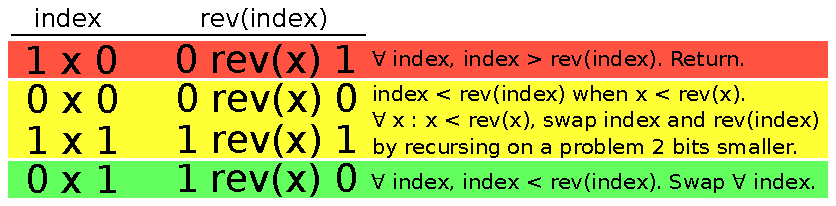
\includegraphics[width=4.5in]{cartoons/unrolled.pdf}
\caption{{\bf Illustration of the unrolled method for bit reversal.}
  All possible bit strings where {\tt index < rev(index)} are found at
  compile time by beginning with the most significant bit remaining
  and least significant bit remaining and progressing inward
  recursively. Bit strings of the form {\tt 1~x~0} will never be less
  than their reverse (highlighted in red). Bit strings of the form
  {\tt 0~x~1} will always be less than their reverse (highlighted in
  green). Bit strings of the form {\tt 0~x~0} and {\tt 1~x~1} will
  only be less than their reverse when {\tt x < rev(x)} (highlighted
  in yellow).
  \label{figure:unrolled}}
\end{figure}

Para problemas pequeños, este método plantilla-recursivo "desenrollado" es
muy eficiente. Sin embargo, una desventaja del método es que en
Problemas, se generará una gran cantidad de código, lo que grandes tiempos de compilación y también puede significar que el orden de la operaciones de intercambio no serán optimizadas de manera efectiva compilador. De hecho, puede que no haya una orden de caché eficiente para visitar los índices están siendo intercambiados porque los índices invertidos de bits saltan alrededor. Así, a menos que el compilador posea conocimientos matemáticos sobre los swaps
(que permite al compilador transformar el código en uno de los otros algoritmos listados), el método desenrollado es mediocre eficiencia en los grandes problemas no justificará su sustancial tiempos de compilación.
\paragraph{Cache-oblivious recursive bit-reversed permutation:}
Cuando el número de bits $ b $ es par, una cadena de bits de índice puede ser
Dividido en dos secuencias de bits de igual tamaño de $\frac{b}{2}$ bits cada uno:{\tt index = x ~ y}. El índice invertido sería {\tt rev(index) ~ = ~ rev(y) ~ rev(x)}. Esto se puede calcular en tres pasos: en primer lugar, invertir los bits menos significativos (que forman {\tt y}) a producir {\tt x ~rev(y)}. En segundo lugar, intercambiando los bits más significativos
Formando {\tt x} con los bits menos significativos formando {\tt rev(y)},
Produciendo así {\tt rev(y) ~ x}. En tercer lugar, repitiendo el primer paso y invirtiendo los bits menos significativos (que en este punto contienen {\tt X}) para producir {\tt rev(y) ~ rev(x) ~ = ~ rev(índice)}.

Esta técnica recursiva no sólo es útil para calcular una index: también se puede utilizar para realizar todo el bit invertido permutación de manera recursiva con operaciones localizadas que no es necesario ajustar el tamaño de la caché. El primer y el tercer paso son se realizan de manera idéntica entre sí: para todo lo posible secuencias de bits significativas, realizan un bit local más pequeño, invertido permutación de tamaño $ \ frac {b} {2} $. Estos bits recursivos invertidos todas las permutaciones se aplicarán a bloques mucho más pequeños y contiguos de memoria, mejorando así el rendimiento de la memoria caché. El segundo paso, en el que las cadenas de bits más significativas y menos significativas son inversa corresponde a una transposición matricial, con la mayor bits significativos correspondientes a las filas de la matriz y los menos bits significativos correspondientes a las columnas (utilizando el estilo {\ tt C} organización de orden de orden de filas). Puesto que {\ tt x} y {\ tt y} usan iguales número de bits, este intercambio corresponde a una transposición de un cuadrado matriz, que puede realizarse en su lugar. Además, una cache-oblivious algoritmo (lo que significa que está cerca de la óptima tiempo de ejecución posible para cualquier organización de caché jerárquica) para la matriz se conoce la transposición, que lleva a cabo la transposición en y otras subdivisiones \ cite {prokop: cache}. Por lo tanto, la permutación invertida en bits puede reducirse a bit invertido más pequeño permutaciones en bloques contiguos de memoria y una matriz cuadrada transposición ({\bf Figura ~\ref{figura: recursivo}}).
\begin{figure}
\centering
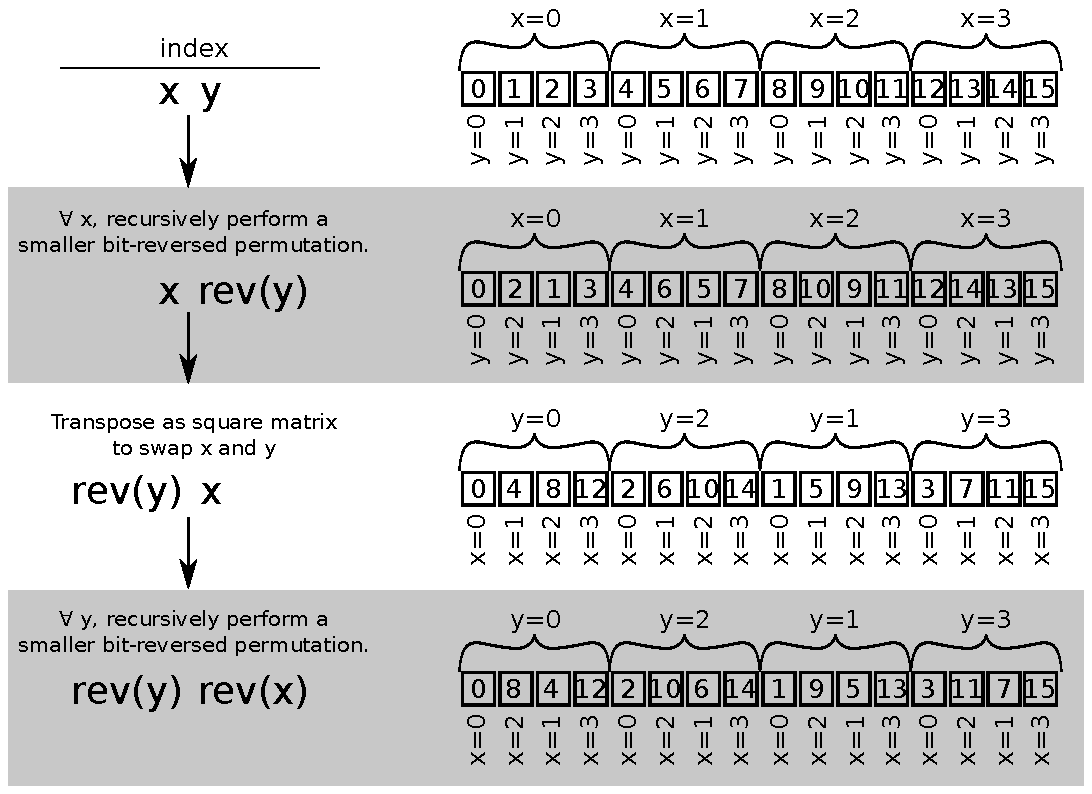
\includegraphics[width=5in]{cartoons/recursive.pdf}
\caption{{\bf Illustration of recursive bit-reversed permutation.} A
  bit-reversed permutation on $b$ bits is performed as several smaller
  bit-reversed permutations on $\frac{b}{2}$ bits, an in-place
  transposition of a square matrix and another batch of smaller
  bit-reversed permutations on $\frac{b}{2}$ bits. The spatial
  locality of each of these steps yields a cache-performant algorithm.
  \label{figure:recursive}}
\end{figure}

When the number of bits $b$ is odd, then a single even-odd permutation
can be performed first: Reversing {\tt index = x~y~z} where {\tt z}
consists of a single bit yields {\tt rev(index) = z~rev(y)~rev(x)}. An
even-odd permutation produces {\tt z~x~y}. Applying a $b-1$
bit-reversed permutation when {\tt z}=0 and another $b-1$ bit-reversed
permutation {\tt z}=1 will yield {\tt z~rev(y)~rev(x)}. This even-odd
permutation for preprocessing when $b$ is odd will slightly increase
the runtime in that case (this even-odd permutation is also performed
out of place by using a buffer of size $\frac{n}{2}$).

The runtime of the recursive method is defined by the recurrence $r(b)
= 2 \cdot 2^{\frac{b}{2}} \cdot r(\frac{b}{2}) + 2^b$. This recurrence
has closed form $r(b) = 2^{b-3} \cdot b \cdot c + 2^b \cdot (b-1)$,
where $c$ is a constant. Thus $r(b) \in \Theta(2^b \cdot b) = \Theta(n
\log(n))$.

In spite of the flaws in the unrolled closed form when $b \gg 1$, it
is very efficient for small to moderate-sized problems (\emph{e.g.},
$b \leq 14$, which corresponds to $n \leq 16384$); therefore, it is an
ideal base case for the recursive method. The recursive calls can be
made using template recursion, thereby enabling the compiler to
optimize code shared by these recursive calls. This recursive method
generalizes to a semi-recursive method, which not only calls the
unrolled implementation when the number of bits is below a threshold,
it also calls the unrolled implementation when the recursion depth
passes beyond a threshold. This can allow the compiler greater
optimizations, because all of the template-recursive bit-reversed
permutations can be inlined (for larger recursion depths, compilers do
not always inline all of the code, which can be seen by the much
higher compilation times when decorating the recursive bit-reversed
permutation function with {\tt attribute~(\_\_always\_inline\_\_)},
which forces inlining in {\tt g++} and {\tt clang}). Note that a
semi-recursive method that only allows a single recursion will have
runtime $r(b) = 2 \cdot 2^{\frac{b}{2}} \cdot 2^{\frac{b}{2}} + 2^b$,
because the recursive calls $r(\frac{b}{2})$ will be replaced with the
unrolled method runtime, $2^{\frac{b}{2}}$. Therefore, the runtime of
that semi-recursive method becomes $2\cdot 2^b + 2^b \in \Theta(2^b) =
\Theta(n)$.

An advantage of the recursive method over COBRA is that (at least when
the number of bits $b$ is even, $\frac{b}{2}$ is even, \ldots until
the base case size or recursion limit are reached) it can be performed
completely in place and without a buffer. Because the recursive method
reduced bit-reversed permutation to smaller bit-reversed permutations
(each of which are performed independently and in an in-place manner)
and to a square matrix transposition, the method is well suited to
parallelization via SIMD, multiple cores, or by broadcasting over
GPUs; parallelization of COBRA would require duplicate buffers for
each parallelization in order to prevent race conditions.\newline

The asymptotic runtimes for all methods are shown in {\bf
  Table~\ref{table:theoretical-runtimes}}.
\begin{table}[ht!]
  \centering
  \small
  \scalebox{0.88}{
    \begin{tabular}{c|cccccccc}
      & Stockham & Bitwise & Bytewise & Pair bitwise & COBRA & Unrolled & XOR & Recursive \\
      \hline
      %& \multicolumn{3}{c}{$d$ known at compile time} \\
	  {\bf Runtime} & \multirow{2}{*}{$n \log(n)$} & \multirow{2}{*}{$n \log(n)$} & \multirow{2}{*}{$n \log(n)$} & \multirow{2}{*}{$n \log(n)$} & \multirow{2}{*}{$n + \frac{n}{t} \log(\frac{n}{t})$} & \multirow{2}{*}{$n$} & $n$ or & $n$ or \\ 
          (asymptotic) & & & & & & & $n \log(\log(n))$ & $n \log(n)$\\
	  \hline
    \end{tabular}
  }
  \caption{{\bf Theoretical runtimes.} The asymptotic runtimes for
    each algorithm are given. Note that the algorithms with lowest
    theoretical runtime are not necessarily superior in practice: For
    example, the bitwise and bytewise methods are both $\in \Theta(n
    \log(n))$, but the bytewise method has a superior runtime constant
    because it uses a table to reverse words using 8 bits at a
    time. Likewise, the pair bitwise, COBRA, and recursive methods all
    accesses memory in more contiguous, local fashions and therefore
    have superior cache locality. For the COBRA method, $t$ is the
    buffer size used. The runtime of the inductive XOR method will be
    either $\in \Theta(n)$ (when count leading zeros is $\Theta(1)$)
    or $\Theta(n \log(\log(n)))$ (when count leading zeros cannot be
    performed in hardware, and thus requires $\in
    \Theta(\log(\log(n)))$ steps). The recursive method will require
    $\in \Theta(n \log(n))$ steps in general, but can be sped up to
    $\in \Theta(n)$ steps when using a semi-recursive approach, which
    limits the recursion depth.}
  \label{table:theoretical-runtimes}
\end{table}

\section*{Results}
Todos los métodos se implementaron en {\tt C ++ 11}, haciendo uso de la plantilla recursión, junto con las variables {\tt constexpr} y funciones. Los tiempos de ejecución se compararon, comparando todos los compilando con {\tt clang++ 3.8.0} y {\tt g++ 6.2.0}. En ambos compiladores, la compilación se optimizó con flags {\tt –Ofast -march = nativo -mtune = nativo}. Para no arriesgar el aliasing del puntero interferencia entre diferentes puntos de referencia, cada algoritmo y el tamaño de entrada se comparó en un archivo separado de {\ tt main.cpp}. Compilar veces con {\tt clang ++} se trazan en {\bf Figura~\ref{fig: clang++_compile_times}} tiempos de compilación con {\tt g++} en {\bf Figura~\ref{fig: g++_compile_times}}. Todos los métodos fueron aplicados a matrices de tipo {\tt std::complex<double>}, ya que nuestro primario la motivación de realizar una rápida permutación de bits invertidos radica en evaluando la idoneidad de los métodos para la implementación de FFT. Tenga en cuenta que las prestaciones individuales de los métodos pueden variar ligeramente cuando tipos de datos con diferentes tamaños (\emph{por ejemplo.}, {\tt int} o {\tt float}).

Tanto para los métodos COBRA in situ como fuera de lugar, el tamaño del búfer
Se optimizó para cada tamaño de problema. La memoria recursiva caché-olvidada
Método utilizó una base de casos de tamaño $ b \ leq 9 $, en cuyo punto
Calculó la forma cerrada desenrollada de la permutación invertida en bits de
tamaño. El tiempo de ejecución no era muy sensible a esta elección del caso base tamaño; Esto es una reminiscencia del tamaño del caso base usado en
Transposición matricial de la memoria cache-oblivious, donde se utiliza
Amortizar el costo de las recursiones, asegurando el costo computacional del caso base no es trivial.

Los tamaños de problemas comparados varían entre $n = 2^8$ (lo que requiere $\Approx 4$ KB para almacenar) a $n = 2^{30}$ (lo que requiere $\approx
16.4$ GB para almacenar). Todas las mediciones se hicieron un promedio de 100 carreras, y runtimes se informan en segundos por elemento (\ emph {i.e.}, El total tiempo transcurrido para la permutación invertida en bits dividido por $ n $). La CPU especificaciones del ordenador utilizado para la evaluación comparativa se
{\bf Table~\ref{tabla: cpu_spec}}. Los tiempos de ejecución para todas las pruebas, compilados con {\tt clang++} y {\tt g++} se muestran en {\bf
  Figura~\ref{fig: clang++_runtimes}} y {\bf
  Figura~\ref{fig: g++_runtimes}}, respectivamente.

Con el fin de medir su naturaleza inherentemente paralela, versiones del método semi-recursivo también fueron implementadas y comparado: El primero de estos múltiples núcleos a través de OpenMP y el {\tt -fopenmp} opción del compilador. Esta implementación de OpenMP utiliza {\tt \#pragma omp parallel for} para permitir las llamadas recursivas (que se puede implementar a través de la forma cerrada desenrollada ya que sólo una recursión está permitido) en paralelo. La segunda versión paralela adapta el método semi-recursivo para usar la GPU a través de la CUDA Kit de herramientas Esta implementación de GPU permite dos recursiones y es codificado por $ b = 24 $ (requiere que los índices intercambiados se almacenen en una matriz, que se transmite a través de la GPU). $ B = 24 $ fue elegido porque era el problema más grande que encajaría totalmente en la GPU tal que $B$ es divisible por 4 (los problemas divisibles por 4 pueden ser expandidos por dos
Recursiones sin realizar una permutación impar
Preprocesamiento). Esta implementación de CUDA también realiza la
transposición en la GPU \ cite {harris: cuda}, y por lo tanto paraleliza
tanto las llamadas recursivas como la transposición (esto tiene un
beneficio de solo tener que mover datos a la GPU una vez). Tanto el OpenMP
y las versiones paralelas de la GPU fueron compiladas con {\tt g ++} (y la
versión de la GPU utilizada {\tt nvcc}), debido al apoyo limitado hasta la fecha para tanto OpenMP como CUDA en {\ tt clang ++}. Estas versiones paralelas son en comparación con los mejores métodos de un solo hilo en {\bf
  Figura~\ref{fig: g++_parallel_runtimes}}
\begin{table}[ht!]
  \centering
  \begin{tabular}{cccccc} L1d &  L1i &    L2 &      L3 & MAX\_SPEED &   RAM \\
\midrule
 32K &  32K &  256K &  15360K &    3.8Ghz &  65GB \\
\end{tabular}
\caption{ {\bf CPU specification used for benchmarking.} The size of
  the L1 data cache, the L1 instruction cache, the L2 cache, the L3
  cache, and the clockspeed as well as the RAM-size of the computer
  used for benchmarking are shown. To relate this to the
  benchmark-results we have shown, note that $32$K can contain hold an
  array of $n=2^{11}$ elements of type {\tt std::complex<double>},
  $256$K can hold $n=2^{14}$ elements, and $15360$K can hold $n=2^{20}$
  elements. The $65$GB of RAM can hold $n=2^{31}$ elements. 
  \label{table:cpu_spec}
}
\end{table}

\begin{figure}[ht!]
\centering
\begin{tabular}{cc}
  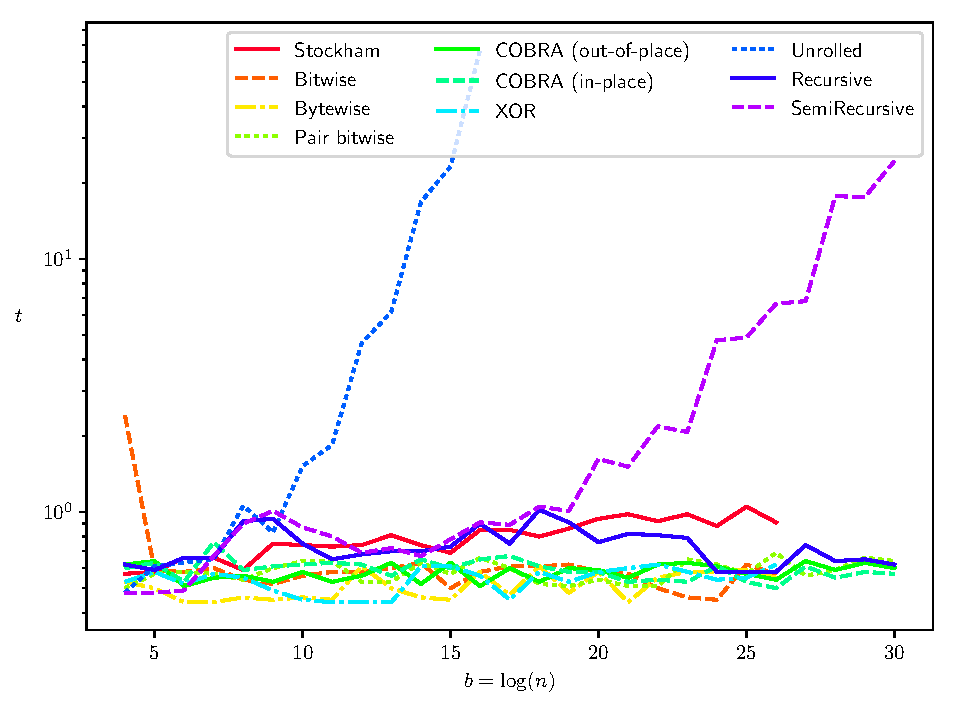
\includegraphics[width=4.5in]{results/clang++_compile_times.pdf}
\end{tabular}
\caption{{\bf Compile times with {\tt clang++}}. For each method, the
  compile time for the bit-reversed permutations of various sizes are
  plotted. Note that the $t$-axis is scaled logarithmically.  Runtimes
  for each method are depicted in figure \ref{fig:clang++_runtimes}.
  Note that UnrolledShuffle has been exluded from compilation for
  $b>16$, since the size of the executables, as well as compile times
  would get unreasonably big.
  \label{fig:clang++_compile_times}	
}
\end{figure}

\begin{figure}[ht!]
\centering
\begin{tabular}{cc}
  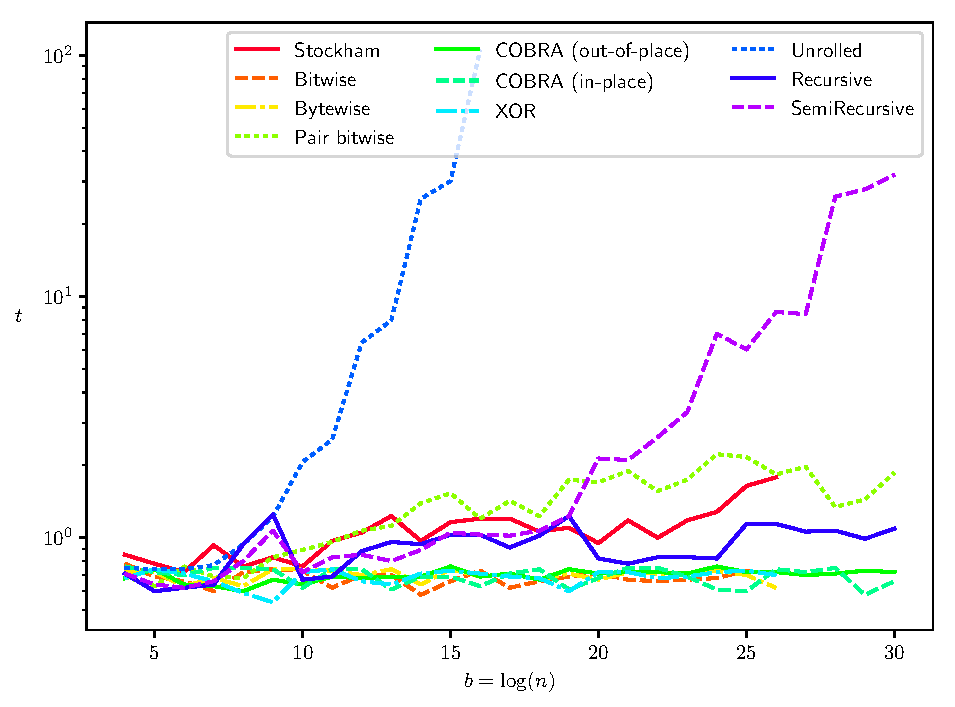
\includegraphics[width=4.5in]{results/g++_compile_times.pdf}
\end{tabular}
\caption{{\bf Compile times with {\tt g++}}. For each method, the
  compile time for the bit-reversed permutations of various sizes are
  plotted. Note that the $t$-axis is scaled logarithmically.  Runtimes
  for each method are depicted in figure \ref{fig:g++_runtimes}. Note
  that UnrolledShuffle has been exluded from compilation for $b>16$,
  since the size of the executables, as well as compile times would
  get unreasonably big.
  \label{fig:g++_compile_times}	
}
\end{figure}

\begin{figure}[ht!]
\centering
\begin{tabular}{cc}
  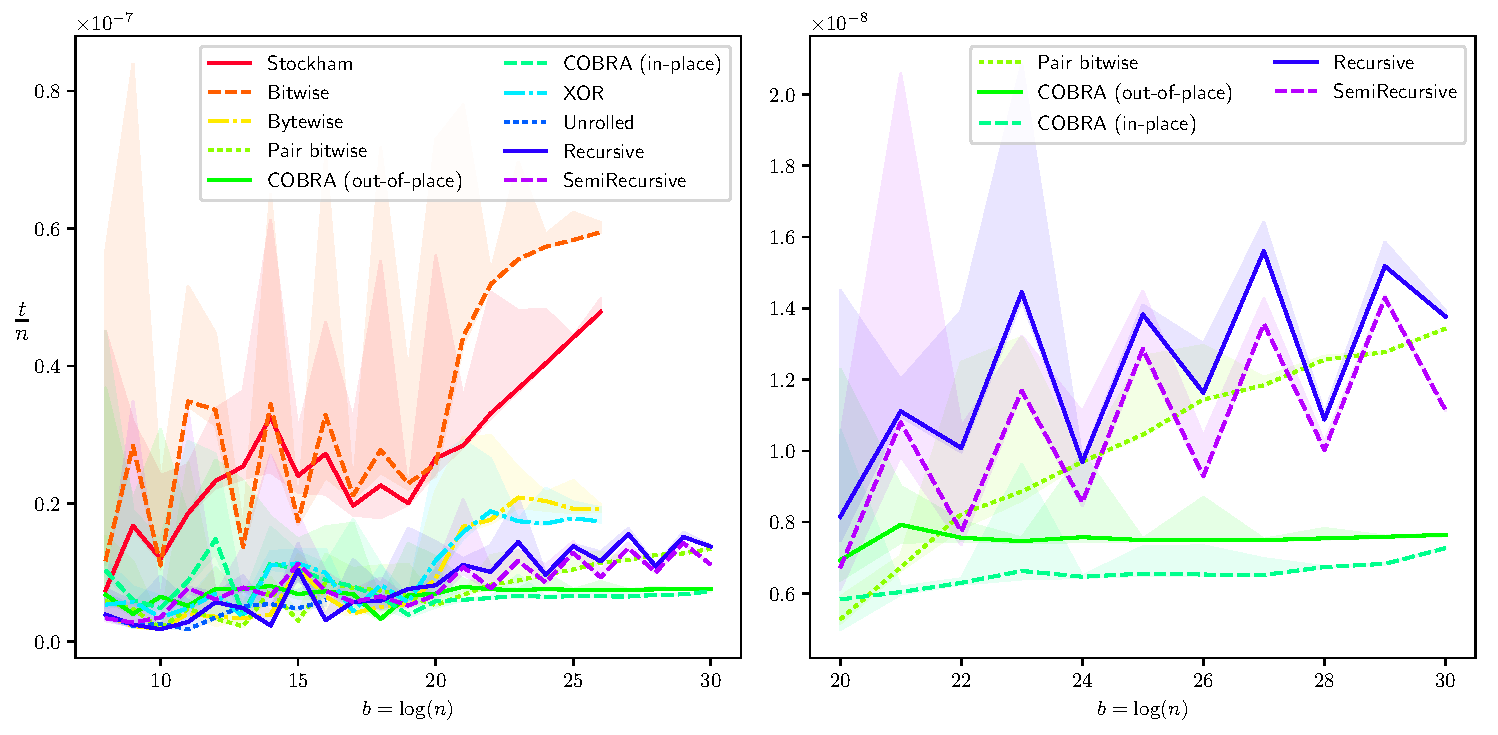
\includegraphics[width=6in]{results/clang++_run_times.pdf}
\end{tabular}
\caption{{\bf Runtimes per element with {\tt g++}}. For each method,
  bit-reversed permutations of various sizes are performed. For each
  method and on each problem size, 100 replicate runtimes (in seconds)
  were measured, and the average runtime per element (\emph{i.e.},
  elapsed time divided by $n = 2^b$) are plotted. The shaded areas
  around each series depict the minimum and the maximum runtimes in 
  all of the 100 replicates. The left panel shows all
  methods from $b=4$ to $b=30$ and the right panel shows only the
  highest performance series on larger problems $b=20$ to $b=30$. The
  methods with poor performance on large problem sizes (Stockham,
  bitwise, bytewise and XOR) have been excluded from benchmarking for
  $b>26$.
  \label{fig:clang++_runtimes}	
}
\end{figure}

\begin{figure}[ht!]
\centering
\begin{tabular}{cc}
  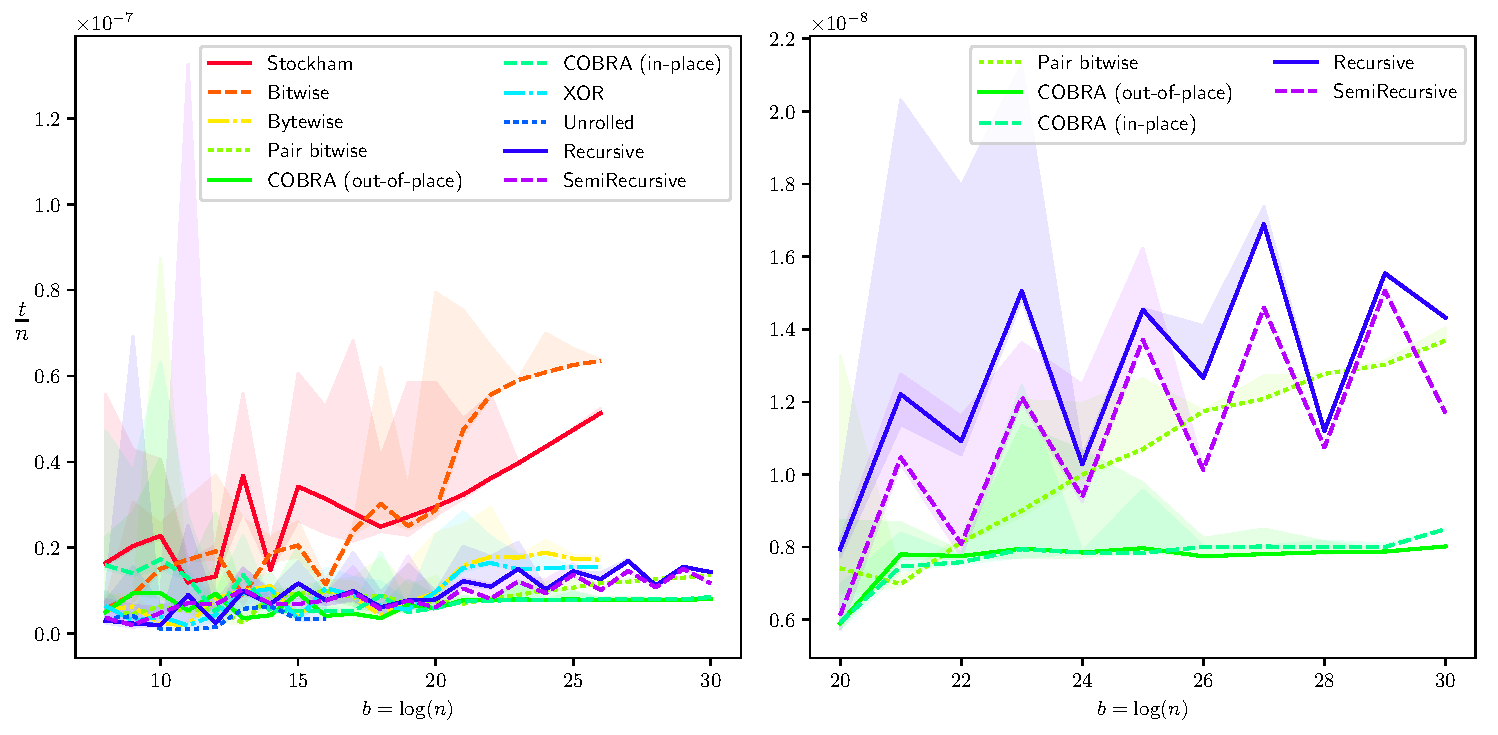
\includegraphics[width=6in]{results/g++_run_times.pdf}
\end{tabular}
\caption{{\bf Runtimes per element with {\tt g++}}. For each method,
  bit-reversed permutations of various sizes are performed. For each
  method and on each problem size, 100 replicate runtimes (in seconds)
  were measured, and the average runtime per element (\emph{i.e.},
  elapsed time divided by $n = 2^b$) are plotted. The shaded areas
  around each series depict the minimum and the maximum runtimes in 
  all of the 100 replicates. The left panel shows all
  methods from $b=4$ to $b=30$ and the right panel shows only the
  highest performance series on larger problems $b=20$ to $b=30$. The
  methods with poor performance on large problem sizes (Stockham,
  bitwise, bytewise and XOR) have been excluded from benchmarking for
  $b>26$.
  \label{fig:g++_runtimes}	
}
\end{figure}

\begin{figure}[ht!]
\centering
\begin{tabular}{cc}
  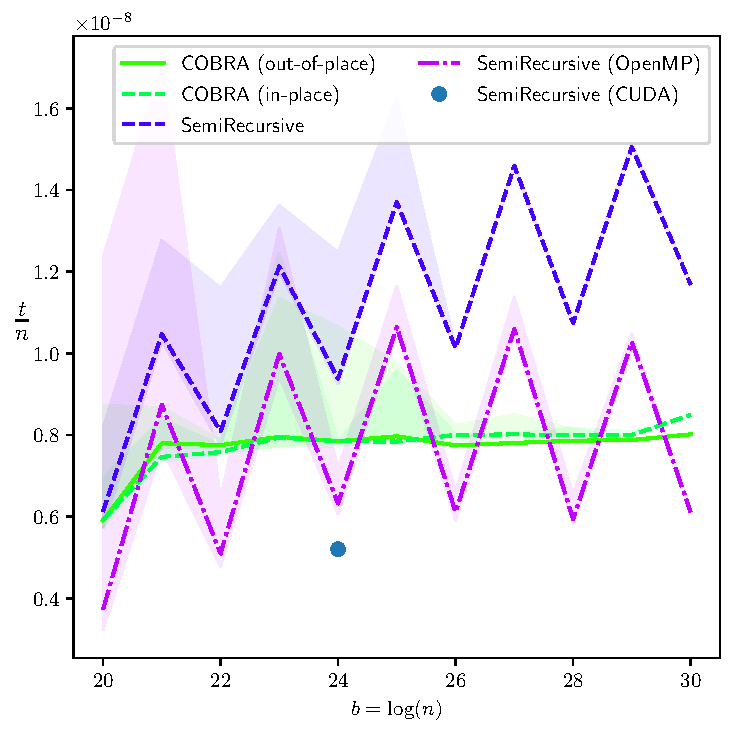
\includegraphics[width=6in]{results/open_mp_performance.pdf}
\end{tabular}
\caption{{\bf Performance gains from parallelization}. Benchmarks were
  repeated from the right panel of {\bf
    Figure~\ref{fig:g++_runtimes}}, but with the inclusion of a
  parallelized versions of the semi-recursive method. Because of the
  semi-recursive methods inherently parallel nature, OpenMP easily
  results in faster performance. Likewise, broadcasting operations
  over the GPU (via CUDA) achieves even greater parallelism.
  \label{fig:g++_parallel_runtimes}
}
\end{figure}

\section*{Discussion}
Con los dos {\tt g++} y {\tt clang ++}, el Stockham e ingenuo bitwise los métodos de barajado tienen un rendimiento aproximadamente similar entre sí y son los métodos menos eficientes investigados aquí. El método de Stockham
es un procedimiento fuera de lugar (aumentando así la carga sobre la caché)
y realiza más operaciones de intercambio que el barajado de bits; sin embargo, el método de Stockham accede a los datos mediante elementos pares e impares y, por tanto, acceso a los datos de una manera aproximadamente contigua, mientras que el bit a bit método accede a los datos de una manera menos contigua porque accede al índice {\tt rev (i)} en cada iteración.

El método bytewise table y el método XOR consiguen rendimiento entre sí. Ambos métodos escalan considerablemente mejor que los métodos de Stockham y bitwise. Tanto el método de tabla bytewise y el método XOR lograr una inversión de bit más rápida, pero ninguno logra un patrón de acceso de memoria contiguo; Por lo tanto, tampoco es muy caché performante el método XOR propuesto todavía puede utilizarse en zonas en las que la memoria está en una prima (\emph{p. Ej., Sistemas embebidos), ya que rendimiento similar a la tabla de bytes sin almacenar ni accediendo a una tabla de $256$ B.

Para problemas pequeños, el enfoque desenrollado logra esencialmente óptimo
rendimiento, ya que toda la matriz puede caber en la caché L1
y no hay sobrecarga para bucle, inversión de bits o rama
declaraciones. Además, las operaciones pueden ser compiladas para usar
direccionamiento de modo inmediato en el código de ensamblaje, lo que
los índices intercambiados se codifican de forma nativa en las instrucciones de montaje
y no necesitan ser codificados en una matriz separada. El tiempo de ejecución
beneficio de este método desenrollado no se extiende a problemas mayores
(Porque la matriz no encaja en las caché L1 o L2) y la
tiempo de compilación del método desenrollado se vuelve muy caro (aproximadamente
100 segundos cuando $b = 16$ para ambos {\tt g ++} y {\tt clang++}).

los algoritmos más eficaces en problemas grandes son los diseñados
con la caché en mente: esto incluye el par de método bitwise, el
COBRA (tanto en el lugar como fuera de lugar), y el método recursivo
y su variante semi-recursiva. La recursiva y métodos semi-recursivos cuando se aplican a problemas con una número de bits, ya que no es necesario realizar una permutación impar preprocesado (esto da como resultado un patrón de dientes de sierra en los tiempos de de grandes problemas). El método semi-recursivo alcanza ligeramente mayor rendimiento que el método recursivo, pero a costa de un mayor tiempo de compilación (entre 10 a 13 segundos cuando $ b = 28 $ usando tanto {\tt g++} como {\tt clang++}). Para problemas más pequeños, el método COBRA fuera de lugar es menos eficiente que su variante in situ, debido a la mayor carga en la caché de utilizar el doble de
memoria. Sin embargo, para problemas más grandes, un mayor rendimiento es
logrado por el método COBRA fuera de lugar, ya que el método fuera de lugar
método copia valores a través de un búfer, mientras que el método in situ intercambia valores a través del búfer; Por lo tanto, el método in situ debe copiar al y luego intercambiar entre el búfer y la matriz, luego intercambiar
Los cambios resultantes en el búfer de nuevo en la matriz.

El método de inversión de bits de par realiza más operaciones de intercambio, pero con mayor localidad y sin el uso de un buffer de resultados (tal
requerido por algoritmos fuera de lugar como Stockham). El par a bit
método COBRA, y los métodos recursivo y semi-recursivo los métodos funcionan de manera similar para problemas grandes; El fuera de lugar el método COBRA funciona ligeramente mejor para problemas más grandes, pero su las ganancias de rendimiento se silencian cuando el tamaño del búfer de la matriz no es optimizado para la CPU. Hay pequeños aumentos en el tiempo de elemento en los límites de caché, sobre todo en el límite de la caché L3 en $b = 18$ para los métodos in situ y en $b = 17$ para métodos fuera de lugar.

A diferencia de los métodos COBRA, que consiguen su rendimiento a través de una matriz buffer, los métodos recursivos y semi-recursivos son inherentemente caché eficiente y no utilizar dicho tampón; Por lo tanto, son adecuados para paralelismo {\bf Figura~\ref{fig: g++_parallel_runtimes}} muestra la un fuerte beneficio de rendimiento que puede lograrse añadiendo paralelismo de grano grueso a través de OpenMP o añadiendo grano fino paralelismo con la GPU. Las recursiones no necesitan acceder a ninguna información de otros elementos, por lo que son perfectamente concurrencia (incluyendo el hecho de que las arquitecturas modernas incluyen cachés L1 independientes para cada núcleo de hardware). Este calidad paralelizable a los métodos recursivo y semi-recursivo también podría ser explotado con mayor eficacia mediante la optimización el código de la GPU.

En $b = 24$ en la Figure~\ref{fig: g++_parallel_runtimes}, el tiempo de ejecución de el método no paralelo más rápido requiere menos de $8 \times
{10} ^ {-9}$ segundos por elemento, o aproximadamente $0,13$ segundos en total. En comparación, la variante OpenMP del método semi-recursivo requiere
Aproximadamente $0.1$ segundos, y la variante de GPU de la semi-recursiva
Método requies $0.08$ segundos. Como punto de referencia, el {\tt numpy} FFT (que utiliza la biblioteca {\tt FFTPACK}) toma aproximadamente 2 segundos para problemas de ese tamaño. El ingenuo enfoque bit a bit requiere aproximadamente 1 segundo, lo que indica que alrededor del 50 \% del tiempo total de ejecución FFT en la permutación invertida en bits, lo que significa que la velocidad de usar estos métodos de permutación de bits invertidos más rápido es no trivial; Aunque el código de mariposa FFT realiza más manipulaciones sofisticadas de números complejos, lo hace de contiguo, haciendo que la permutación invertida sea más importante de lo que puede parecer. Además, utilizando este método semi-recursivo para realizar la FFT completa en la GPU no sólo se beneficiaría de la ejecución pequeñas operaciones de mariposa FFT en paralelo, también reducir el tiempo de ejecución de la permutación invertida en bits evitando la costo de copiar datos desde y hacia la GPU.

Aparte de la capacidad de paralelizar los métodos recursivos, sus beneficio proviene del hecho de que alcanzan un alto rendimiento sin tuning para una arquitectura de caché específica (que hemos encontrado influye sustancialmente en la eficiencia de COBRA métodos). Específicamente, el método recursivo no tiene memoria caché. Cuando junto con un método óptimo de cache-oblivious para la matriz transposition \cite{prokop: cache}, que garantiza bastante contiguo accesos de memoria sin ningún conocimiento de la arquitectura de caché. Me gusta el método recursivo, la estrategia semi-recursiva tampoco utiliza una búfer con el tamaño ajustado para el funcionamiento del escondrijo; sin embargo, el semi-recursivo no es caché-oblivious, porque los grandes problemas pueden ser reducidos a problemas de permutación de bits invertidos menores que todavía no encajar en la caché. El método recursivo no sólo es interesante para investigación futura que investigue el beneficio de rendimiento de paralelizarlo, el hecho de que logra un alto rendimiento sin el ajuste de caché específico de la arquitectura sugiere que es un en la búsqueda de una memoria caché optimizada
permutación.
\section*{Availability}
All {\tt C++11} source code accompanying this paper, preliminary GPU
implementation of the recursive algorithm, as well as benchmarking
scripts, and the \LaTeX\ code for the paper itself are freely
available (Creative Commons license) at
\url{https://bitbucket.org/orserang/bit-reversal-methods}.\newline

\section*{Acknowledgements}

We are grateful to Thimo Wellner and Guy Liang for their
contributions.\newline 

\noindent This paper was written as part of the master course in
Scientific Computing over the winter semester 2016--2017 at Freie
Universit\"at Berlin, taught by Oliver Serang. Translations of this
paper are also available in the mother tongues of every student:
German, Chinese, Turkish, and Spanish (these are linked by the
repository). %fixme: add these links after the translations are finished

\section*{Author Contributions}
The new algorithms and non-parallel implementations in {\tt C++11}
were created by and the project was supervised by O.S. The
Introduction section was written by X.W. The Methods section and
runtime analysis were performed by by B.A., X.W., and D.W. The OpenMP
implementation was made by O.S. and the GPU variant was made by
B.A. The benchmarks, figures, and Results sections were created by
C.K. The Discussion section was created by X.W. and C.K. Testing and
optimization were performed by B.A. and D.W. Final benchmarks were
done by C.K., L.I., T.C., and O.S.\newline

% at end of this section:
\noindent Excluding the senior authors (O.S. and T.C.), the author
order was chosen by a secret ballot among the students.

% bibliography:
\bibliographystyle{unsrt}
\bibliography{refs}


\end{document}

